\begin{figure}[H]
    \thispagestyle{empty}
    \centering
    \rotatebox{90}{
        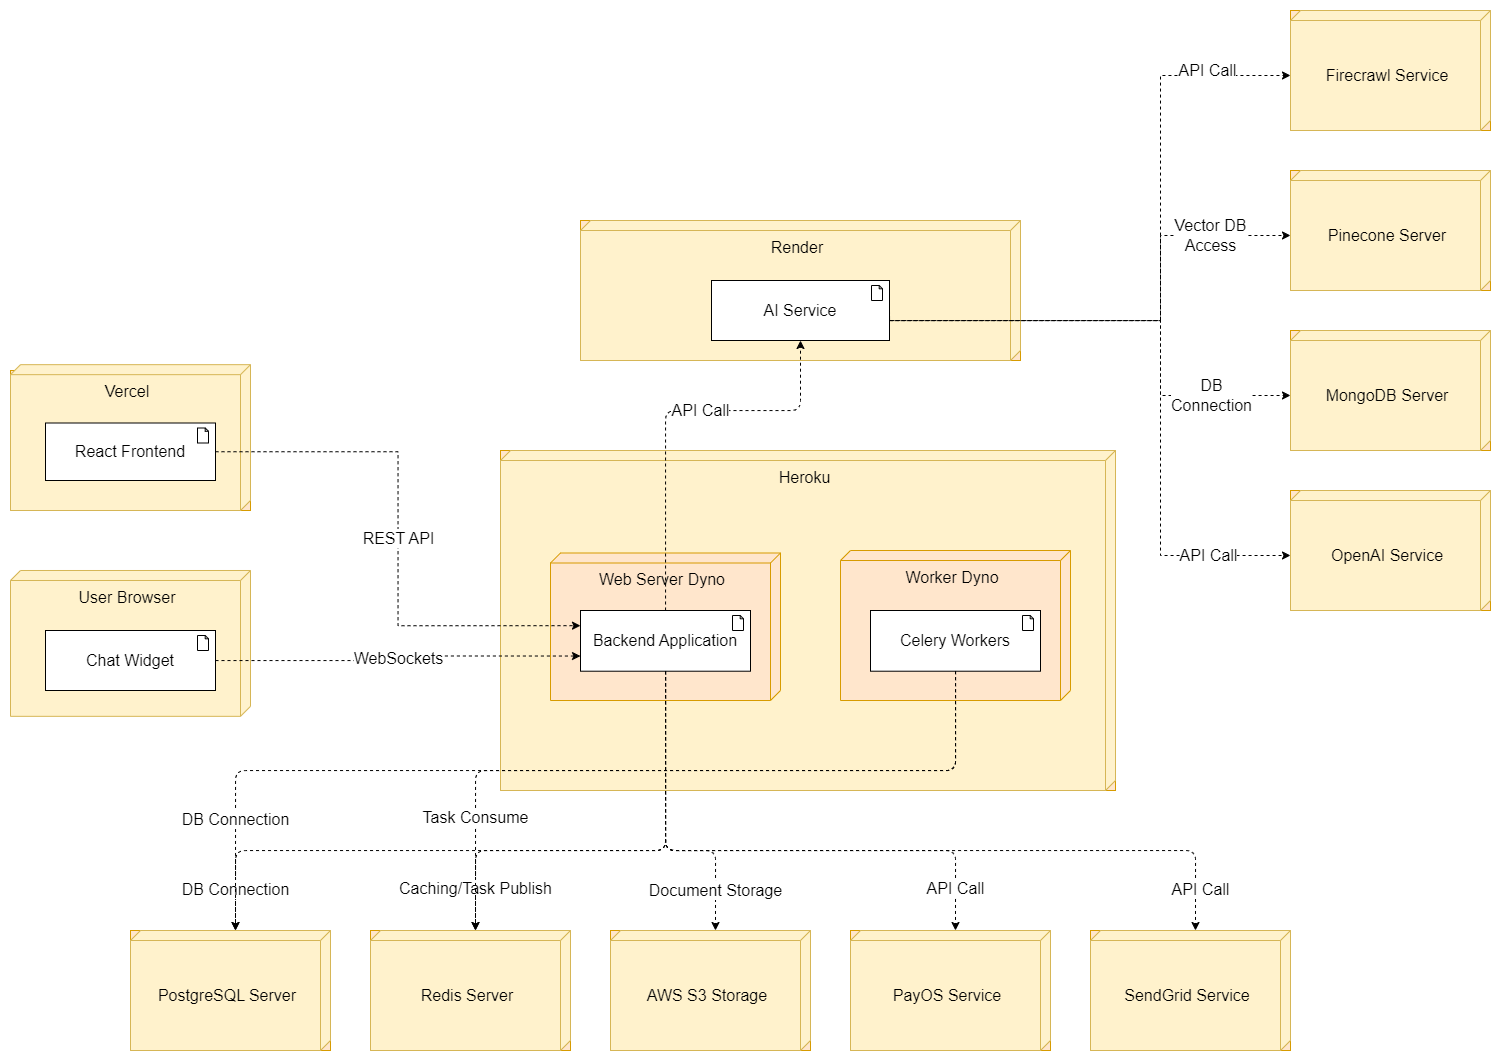
\includegraphics[height=0.9\textwidth, width=0.9\textheight, keepaspectratio]{Dg_System/deployment.png}
        % \includesvg[height=0.9\textwidth, width=0.9\textheight, keepaspectratio]{Dg_System/deployment.drawio.svg}
        }
    \rotatebox{90}{
        \parbox{\textwidth}{
            \centering
            \caption{Sơ đồ triển khai hệ thống}
        }
    }
\end{figure}

Sơ đồ triển khai hệ thống, như được minh họa trong hình 114, mô tả chi tiết cách thức các thành phần phần mềm của ứng dụng được phân bổ và thực thi trên các nút hạ tầng vật lý hoặc ảo trong môi trường vận hành thực tế. Sơ đồ này làm rõ các nền tảng dịch vụ được sử dụng và mối quan hệ tương tác giữa chúng. \\

\textbf{Nền tảng Vercel (Vercel Platform):} Nền tảng Vercel được lựa chọn để triển khai thành phần giao diện quản trị của hệ thống.
\begin{itemize}
    \item \textbf{Ứng dụng React Frontend:} Đây là ứng dụng đơn trang dành cho quản trị viên và nhân viên hỗ trợ. Ứng dụng này giao tiếp với Ứng dụng Backend trên nền tảng Heroku thông qua giao diện REST API để trao đổi dữ liệu và thực thi các yêu cầu nghiệp vụ.
\end{itemize}

\textbf{Trình duyệt Người dùng (User Browser Environment):} Đây là môi trường thực thi phía người dùng cuối, nơi họ tương tác trực tiếp với tiện ích chatbot.
\begin{itemize}
    \item \textbf{Tiện ích Chat (Chat Widget):} Thành phần giao diện người dùng dạng nhúng, được tích hợp vào website của khách hàng. Tiện ích chat thiết lập kết nối WebSocket trực tiếp đến ứng dụng backend trên Heroku để đảm bảo việc gửi và nhận tin nhắn diễn ra tức thời, mang lại trải nghiệm hội thoại thời gian thực.
\end{itemize}

\textbf{Nền tảng Heroku (Heroku Platform):} Heroku, một Nền tảng dưới dạng Dịch vụ (PaaS), đóng vai trò là môi trường triển khai chính cho các thành phần backend cốt lõi của hệ thống. Các thành phần này được thực thi dưới dạng các quy trình (dynos) chuyên biệt:
\begin{itemize}
    \item \textbf{Web Server Dyno (Chứa Ứng dụng Backend - Backend Application):} Dyno này chịu trách nhiệm xử lý các yêu cầu HTTP đến từ Ứng dụng React Frontend và quản lý các kết nối WebSocket từ tiện ích chat. Bên trong dyno này là ứng dụng backend chính (phát triển bằng Django), bao gồm các module dịch vụ xử lý logic nghiệp vụ của hệ thống. Web Server Dyno tương tác với nhiều dịch vụ và máy chủ khác, bao gồm: Máy chủ PostgreSQL để truy vấn cơ sở dữ liệu, Máy chủ Redis cho caching và hàng đợi tác vụ, Dịch vụ Lưu trữ AWS S3 để quản lý tệp, các Dịch vụ Bên ngoài như PayOS và SendGrid qua API call, và Dịch vụ AI trên nền tảng Render cũng thông qua API call. Nó cũng xuất bản các tác vụ nền cho Worker Dyno thông qua Redis.
    \item \textbf{Worker Dyno (Chứa Celery Workers):} Dyno này thực thi các tiến trình Celery Workers, chuyên xử lý các tác vụ nền bất đồng bộ. Các tác vụ này được tiêu thụ từ hàng đợi tin nhắn trên Máy chủ Redis, giúp giảm tải cho Web Server Dyno và cải thiện độ phản hồi của ứng dụng. Worker Dyno có thể cần tương tác với Máy chủ PostgreSQL, Redis, và AWS S3 tùy theo bản chất của tác vụ được xử lý.
\end{itemize}

\textbf{Nền tảng Render (Render Platform):} Nền tảng Render được sử dụng để triển khai Dịch vụ Trí tuệ Nhân tạo một cách độc lập.
\begin{itemize}
    \item \textbf{Dịch vụ AI (AI Service):} Thành phần này đóng gói các mô hình ngôn ngữ lớn, logic xử lý ngôn ngữ tự nhiên, và các thuật toán trí tuệ nhân tạo khác. Dịch vụ AI tiếp nhận các yêu cầu xử lý từ Ứng dụng Backend trên Heroku. Để thực hiện nhiệm vụ, Dịch vụ AI tương tác với:
        \begin{itemize}
            \item \textbf{Máy chủ Pinecone (Pinecone Server):} Truy cập cơ sở dữ liệu vector để thực hiện tìm kiếm tương đồng ngữ nghĩa và các tác vụ liên quan đến Retrieval-Augmented Generation (RAG).
            \item \textbf{Máy chủ MongoDB (MongoDB Server):} Kết nối cơ sở dữ liệu để lưu trữ và truy xuất các dữ liệu cần thiết cho hoạt động của AI, ví dụ như thông tin phiên hội thoại AI, logs xử lý AI, hoặc các dữ liệu bán cấu trúc khác.
            \item \textbf{Dịch vụ OpenAI (OpenAI Service):} Gọi API đến dịch vụ của OpenAI để tận dụng các mô hình ngôn ngữ hoặc các năng lực AI tiên tiến khác.
            \item \textbf{Dịch vụ Firecrawl (Firecrawl Service):} Gọi API đến dịch vụ Firecrawl để thu thập dữ liệu từ các trang web, có thể phục vụ cho việc xây dựng hoặc cập nhật cơ sở tri thức.
        \end{itemize}
\end{itemize}

\textbf{Các máy chủ dữ liệu và lưu trữ phụ trợ:} Hệ thống dựa vào một số máy chủ và dịch vụ chuyên dụng để lưu trữ và quản lý dữ liệu:
\begin{itemize}
    \item \textbf{Máy chủ PostgreSQL (PostgreSQL Server):} Nút máy chủ cơ sở dữ liệu quan hệ, nơi lưu trữ dữ liệu có cấu trúc chính của hệ thống. Được truy cập bởi Web Server Dyno và Worker Dyno trên Heroku thông qua kết nối cơ sở dữ liệu trực tiếp.
    \item \textbf{Máy chủ Redis (Redis Server):} Triển khai dịch vụ Redis, đóng vai trò là bộ nhớ đệm, hàng đợi tin nhắn cho Celery giữa Web Server Dyno và Worker Dyno, và có thể hỗ trợ lớp WebSocket.
    \item \textbf{Dịch vụ Lưu trữ AWS S3 (AWS S3 Storage):} Dịch vụ lưu trữ đối tượng trên nền tảng đám mây của Amazon, được Ứng dụng Backend trên Heroku sử dụng để lưu trữ các tài liệu, hình ảnh, và các tệp dữ liệu khác.
    \item \textbf{Máy chủ MongoDB (MongoDB Server):} Như đã đề cập, máy chủ này triển khai cơ sở dữ liệu NoSQL MongoDB, phục vụ chủ yếu cho nhu cầu lưu trữ dữ liệu của Dịch vụ AI trên Render.
    \item \textbf{Máy chủ Pinecone (Pinecone Server):} Như đã đề cập, đây là một cơ sở dữ liệu vector chuyên dụng, được Dịch vụ AI trên Render sử dụng để lưu trữ và truy vấn các vector nhúng hiệu quả.
\end{itemize}

\textbf{Các dịch vụ bên ngoài tích hợp}

Hệ thống tích hợp với các dịch vụ của bên thứ ba thông qua giao diện lập trình ứng dụng (API) để mở rộng chức năng:
\begin{itemize}
    \item \textbf{Dịch vụ PayOS (PayOS Service):} Cổng thanh toán điện tử, được Ứng dụng Backend trên Heroku gọi để xử lý các giao dịch thanh toán và quản lý gói dịch vụ.
    \item \textbf{Dịch vụ SendGrid (SendGrid Service):} Dịch vụ gửi email, được Ứng dụng Backend trên Heroku sử dụng để gửi các email giao dịch và thông báo cho người dùng.
    \item \textbf{Dịch vụ Firecrawl (Firecrawl Service):} Dịch vụ thu thập dữ liệu web, được Dịch vụ AI trên Render tích hợp để bổ sung dữ liệu cho cơ sở tri thức.
    \item \textbf{Dịch vụ OpenAI (OpenAI Service):} Cung cấp các mô hình ngôn ngữ và API trí tuệ nhân tạo, được Dịch vụ AI trên Render sử dụng để tăng cường khả năng xử lý và sinh phản hồi thông minh.
\end{itemize}
